%%% Copyright (C) 2018 Vincent Goulet
%%%
%%% Ce fichier fait partie du projet
%%% «Programmer avec R»
%%% https://gitlab.com/vigou3/programmer-avec-r
%%%
%%% Cette création est mise à disposition selon le contrat
%%% Attribution-Partage dans les mêmes conditions 4.0
%%% International de Creative Commons.
%%% https://creativecommons.org/licenses/by-sa/4.0/

\chapter{RStudio: une introduction}
\index{RStudio|(}
\label{chap:rstudio}

Un environnement de développement intégré (\emph{integrated
  development environment}, IDE) est un progiciel de productivité
destiné au développement de logiciels ou, plus largement, à la
programmation informatique. Il comprend toujours un éditeur de texte
adapté au langage de programmation visé, un environnement de
compilation ou d'exécution du code et, généralement, des outils de
contrôle de versions, de gestion des projets et de navigation dans le
code source.\footnote{%
  À ce compte, GNU~Emacs constitue un environnement de développement
  intégré.} %

Offert au public depuis 2011, RStudio est un IDE convivial conçu
spécifiquement pour l'analyse de données et le développement de
packages avec R. Il est produit par RStudio~Inc.\ et est offert en
version libre ou commerciale, pour une exécution locale
(\emph{desktop}) ou pour une exécution sur un serveur via un
navigateur web.


\section{Installation}
\label{sec:rstudio:installation}

RStudio est disponible à l'identique pour les plateformes Windows,
macOS et Linux. Pour une utilisation locale sur son poste de travail,
on installera la version libre (\emph{Open Source}) de
\link{https://www.rstudio.com/products/rstudio/download/}{RStudio~Desktop}.


\section{Description sommaire}
\label{sec:rstudio:description}

La fenêtre de RStudio se divise toujours en quatre
sous-fenêtres\footnote{%
  Les sous-fenêtres sont appelées \emph{panes} (en anglais) dans
  l'application.} %
--- sauf au lancement, alors que la sous-fenêtre d'édition de code
source n'est pas visible; voir la \autoref{fig:rstudio:rstudiowindow}.
Dans le sens des aiguilles d'une montre en partant en haut à gauche,
on trouve:
\begin{enumerate}
  \index{RStudio!sous-fenêtres}
\item la sous-fenêtre d'édition de code source, avec un onglet par
  fichier de script;
\item le navigateur d'environnement de travail ou d'historique des
  commandes, selon l'onglet sélectionné;
\item le navigateur de fichiers du projet, de packages, de graphiques,
  etc., selon l'onglet sélectionné;
\item la console --- ou ligne de commande --- R.
\end{enumerate}
Au lancement de l'application, la console R occupe toute la gauche de
la fenêtre jusqu'à ce qu'un fichier de script soit ouvert.

\begin{figure}[t]
  %% Capture d'écran et espace additionnel sous l'image
  \includegraphics{images/rstudiowindow-screenshot}
  \vspace{0.5\TPVertModule}

  \begingroup
  \TPoptions{absolute=false}
  %% Identification de la console
  \begin{textblock}{0.5}(2.65,-0.62)
    \large\faLongArrowDown
  \end{textblock}
  \begin{textblock}{2}(2.2,-0.3)
    \footnotesize\sffamily Console R
  \end{textblock}

  %% Identification du navigateur d'environnement
  \begin{textblock}{1}(7.52,-3.65)
    \large\faLongArrowRight
  \end{textblock}
  \begin{textblock}{2.2}(7.95,-3.9)
    \footnotesize\sffamily\raggedright Navigateur d'environnement et d'historique
  \end{textblock}

  %% Identification de navigateur de fichiers
  \begin{textblock}{1}(7.52,-1.65)
    \large\faLongArrowRight
  \end{textblock}
  \begin{textblock}{2.2}(7.95,-1.9)
    \footnotesize\sffamily\raggedright Navigateur de fichiers, packages, graphiques, etc.
  \end{textblock}
  \endgroup
  \caption[Fenêtre de RStudio sous macOS]{Fenêtre de RStudio et trois
    de ses sous-fenêtres au lancement de l'application sous macOS.
    Sous Windows et Linux, la fenêtre comporte également une barre de
    menu.}
  \label{fig:rstudio:rstudiowindow}
\end{figure}

\begin{itemize}
\item Le navigateur d'environnement de travail est particulièrement
  utile pour voir le contenu, les attributs, le type et la taille de
  chaque objet sauvegardé dans la session R. Il permet également de
  visualiser le contenu des objets en cliquant sur leur nom ou sur
  l'icône de grille à droite de leur nom.
\item Il ne peut y avoir qu'un seul processus R (affiché dans la
  console) actif par fenêtre RStudio. Pour utiliser plusieurs
  processus R simultanément, il faut démarrer autant de copies de
  RStudio.
\item La position des sous-fenêtres dans la grille ne peut être
  modifiée. Par contre, chaque sous-fenêtre peut être redimensionnée.
\item On peut modifier la liste des onglets affichés dans les deux
  navigateurs dans les préférences de l'application; voir la
  \autoref{sec:rstudio:configuration}.
\end{itemize}


\section{Projets}
\index{RStudio!projets}
\label{sec:rstudio:projets}

Il est possible d'utiliser RStudio un peu comme un simple éditeur de
texte.
\begin{itemize}
\item On ouvre les fichiers de scripts un à un, soit à partir du menu
  \code{File|Open file...}, soit à partir de l'onglet \code{Files} du
  navigateur de fichiers.
\item Lorsque nécessaire, on change le répertoire de travail de R à
  partir du menu \code{Session}.
\end{itemize}

Pour faciliter l'organisation de son travail, l'ouverture des fichiers
de script et le lancement d'un processus R dans le bon répertoire de
travail, RStudio propose la notion de \emph{projet}.
\begin{itemize}
\item Un projet RStudio est associé à un répertoire de travail de R
  (\autoref{sec:presentation:workspace}).
\item On crée un nouveau projet à partir du menu \code{Project} à
  l'extrémité droite de la barre d'outils ou à partir du menu
  \code{File|New Project...} On a alors l'option de créer un nouveau
  dossier sur notre poste de travail ou de créer un projet à partir
  d'un dossier existant.
\item Lors de la création d'un projet, RStudio crée dans le dossier
  visé un fichier avec une extension \code{.Rproj} contenant diverses
  informations en lien avec le projet. De plus, le projet est
  immédiatement chargé dans RStudio.
\item L'ouverture d'un projet entraine: le lancement d'une session R
  dont le répertoire de travail est celui du projet; le
  chargement du fichier \code{.RData} (le cas échéant); l'ouverture de
  tous les fichiers de scripts qui étaient ouverts lors de la dernière
  séance de travail.
\item Chaque projet dispose de ses propres réglages. On accède à
  ceux-ci via la commande \code{Project Options...} du menu
  \code{Project} de la barre d'outils.
\item L'utilisation d'un projet permet également d'effectuer la
  gestion des versions du code avec Git ou Subversion
  (\autoref{chap:git}) directement depuis RStudio.
\end{itemize}

On trouvera plus d'information sur les projets dans l'aide en ligne
de RStudio.


\section{Commandes de base}
\label{sec:rstudio:commandes}

Comme l'interface de RStudio respecte les standards modernes, je ne
souligne ici que les commandes particulièrement utiles pour la
manipulation des fichiers de script. On accède rapidement à la liste
des commandes les plus utiles via le menu \code{Help} de
l'application.

Les raccourcis clavier sous, d'une part, Windows et Linux et sous,
d'autre part, macOS, diffèrent légèrement. Je fournis ci-dessous
les deux jeux, séparés par le symbole $\bullet$.

\begin{ttscript}{Ctrl-Shift-S $\bullet$ \cmdkey\shiftkey S}
  \index{RStudio!symbole d'affectation}
\item[\code{Alt+-} $\bullet$ \code{\optkey\,-}] insérer le symbole
  d'affectation \verb*| <- | (pour les
  \capsule{https://youtu.be/alGs2KFpBJw}{Mac avec un clavier
    canadien-français}, consulter l'encadré de la
  \autopageref{fig:rstudio:affectation})
\item[\code{Ctrl+Retour} $\bullet$ \code{\cmdkey\,\returnkey}]
  évaluer dans le processus R la ligne sous le curseur ou la région
  sélectionnée, puis déplacer le curseur à la prochaine expression
\item[\code{Ctrl+Shift+S} $\bullet$ \code{\shiftkey\,\cmdkey\,S}]
  évaluer le code du fichier courant en entier dans le processus R
\item[\code{Ctrl+Alt+B} $\bullet$ \code{\optkey\,\cmdkey\,B}]
  évaluer dans le processus R le code source du début du fichier
  jusqu'à la ligne sous le curseur
\item[\code{Ctrl+Alt+E} $\bullet$ \code{\optkey\,\cmdkey\,E}]
  évaluer dans le processus R le code source de la ligne sous le curseur
  jusqu'à la fin du fichier
\item[\code{Ctrl+Alt+F} $\bullet$ \code{\optkey\,\cmdkey\,F}]
  évaluer le code de la fonction courante dans le processus R
\end{ttscript}

À la console --- ou ligne de commande --- R, les raccourcis suivants
sont particulièrement utiles.
\begin{ttscript}{Ctrl-I $\bullet$ \cmdkey\,I}
\item[$\uparrow$ | $\downarrow$] commande
  précédente~|~suivante dans l'historique
\item[\code{Ctrl+}$\uparrow$ $\bullet$ \cmdkey\,$\uparrow$] afficher
  la fenêtre d'historique des commandes
\end{ttscript}

\begin{figure}[t]
  \refstepcounter{dummy}
  \label{fig:rstudio:affectation}
  \begin{emphbox}{\mdseries Symbole d'affectation et
      Mac munis d'un clavier canadien-français}
    Le très pratique raccourci clavier {\optkey\,-} servant à insérer
    le symbole d'affectation ne fonctionne pas avec le clavier
    canadien-français sur les Mac. Cette combinaison de touches sert
    déjà à insérer le symbole «\textbar». C'est en fait un doublon
    puisque ce symbole est principalement associé à la touche
    {\optkey\,/}.

    Il est possible de régler le problème en redéfinissant le
    raccourci clavier associé au symbole d'affectation. Je recommande
    d'utiliser la combinaison {\optkey\,=} puisque le caractère lié
    normalement à cette touche («\code{¬}») n'est d'aucune utilité dans
    R.

    \begin{enumerate}
    \item Accéder à la fenêtre d'édition des raccourcis clavier via le
      menu \code{Tools|Modify Keyboard Shortcuts\dots}.
    \item Dans le champ de recherche en haut, taper les lettres de
      «assignment» jusqu'à ce que la commande \code{Insert Assignment
        Operator} apparaisse.
    \item Cliquer sur la case du raccouci clavier (qui devrait être
      \code{Alt+-} par défaut) pour l'activer. Appuyer sur \optkey\,=
      pour utiliser cette combinaison de touches comme raccourci.
    \item Appuyer sur le bouton \code{Apply} pour activer le raccourci
      et pour fermer la fenêtre de configuration.
    \end{enumerate}
  \end{emphbox}
\end{figure}


\section{Anatomie d'une session de travail (bis)}
\label{sec:rstudio:session}

On reprend ici la description de %
%\capsule{http://youtu.be/xiNnHegDau8}{session de travail} %
la session de travail %
type présentée à la \autoref{sec:presentation:session}, mais en
expliquant comment compléter chaque étape dans RStudio. Sont
intercalés dans les instructions les raccourcis clavier des commandes
RStudio et les accès par les menus.

\begin{enumerate}
\item Lancer RStudio et ouvrir un nouveau fichier de script ou un
  fichier de script existant.
  \begin{trivlist}
  \item
    \makebox[0.38\linewidth][l]{%
      \colorbox{codebg}{\code{Ctrl+Shift+N} $\bullet$ \code{\shiftkey\,\cmdkey\,N}}}
    \hfill
    \makebox[0.58\linewidth][l]{%
      \colorbox{codebg}{\code{File|New File|R Script...}}}
  \item
    \makebox[0.38\linewidth][l]{%
      \colorbox{codebg}{\code{Ctrl+O} $\bullet$ \code{\cmdkey\,O}}}
    \hfill
    \makebox[0.58\linewidth][l]{%
      \colorbox{codebg}{\code{File|Open File...}}}
  \end{trivlist}
\item C'est une bonne pratique de faire du dossier où se trouve son ou
  ses fichiers de scripts le répertoire de travail de R.
  \begin{trivlist}
  \item
    \colorbox{codebg}{\code{Session|Set Working Directory|To Source File Location}}
  \end{trivlist}
\item Composer le code. Lors de cette étape de programmation, on se
  déplacera souvent du fichier de script à la console R afin
  d'essayer diverses expressions. On exécutera également des parties
  seulement du code se trouvant dans le fichier de script.
  \begin{trivlist}
  \item
    \makebox[0.38\linewidth][l]{%
      \colorbox{codebg}{\code{Ctrl+Retour} $\bullet$ \code{\cmdkey\,\returnkey}}}
    \hfill
    \makebox[0.58\linewidth][l]{%
      \colorbox{codebg}{\code{Code|Run Selected Line(s)}}}
  \item
    \makebox[0.38\linewidth][l]{%
      \colorbox{codebg}{\code{Ctrl+1} $\bullet$ \code{\cmdkey\,1}}}
    \hfill
    \makebox[0.58\linewidth][l]{%
      \colorbox{codebg}{\code{View|Move Focus to Source}}}
  \item
    \makebox[0.38\linewidth][l]{%
      \colorbox{codebg}{\code{Ctrl+2} $\bullet$ \code{\cmdkey\,2}}}
    \hfill
    \makebox[0.58\linewidth][l]{%
      \colorbox{codebg}{\code{View|Move Focus to Console}}}
  \end{trivlist}
\item Sauvegarder le fichier de script.
  \begin{trivlist}
  \item
    \makebox[0.38\linewidth][l]{%
      \colorbox{codebg}{\code{Ctrl+S} $\bullet$ \code{\cmdkey\,S}}}
    \hfill
    \makebox[0.58\linewidth][l]{%
      \colorbox{codebg}{\code{File|Save}}}
  \end{trivlist}
  (S'il s'agit d'un nouveau fichier, s'assurer de terminer son nom par
  \code{.R}.) Le nom du fichier dans l'onglet de la sous-fenêtre passe
  du rouge au noir.
\item Sauvegarder, si désiré, l'espace de travail de R avec
  \code{save.image()}\index{save.image@\code{save.image}}. Cela n'est
  habituellement pas nécessaire à moins que l'espace de travail ne
  contienne des objets importants ou longs à recréer.
  \begin{trivlist}
  \item
    \colorbox{codebg}{\code{Session|Save Workspace As...}}
  \end{trivlist}
\item Quitter RStudio de la manière usuelle. Par défaut, RStudio
  devrait demander si l'on souhaite sauvegarder l'espace de travail de
  R. Nous suggérons de ne pas le faire.

  La \autoref{sec:rstudio:configuration} explique comment configurer
  RStudio afin d'éviter de se faire poser la question à chaque
  fermeture de l'application.
\end{enumerate}


\section{Configuration de l'éditeur}
\index{RStudio!configuration}
\label{sec:rstudio:configuration}

Il est possible de configurer plusieurs facettes de RStudio à partir
d'une interface familière. On accède aux options de configuration par
le menu \code{Tools|Global Options...} sous Windows et Linux, et par le
menu standard \code{RStudio|Preferences} (\code{\cmdkey\,,})
sous macOS.

Je recommande d'effectuer les configurations suivantes.
\begin{enumerate}
\item Dans la catégorie des options de configuration générales, régler
  l'option \code{Save workspace to .RData on exit} à \code{Never}, tel
  qu'illustré à la \autoref{fig:rstudio:rstudio-on-exit}. Avec ce
  réglage, l'espace de travail de R ne sera pas sauvegardé à la
  fermeture de RStudio.
\item Dans la catégorie \code{Code} et la sous-catégorie
  \code{Editing}, régler l'option \code{Tab width} à \code{4} afin
  d'indenter le code de quatre caractères par défaut. (Ce réglage fait
  aussi l'objet de l'\autoref{ex:fonctions:rstudio-tab-width}.)
\item Toujours dans la catégorie \code{Code}, mais dans la
  sous-catégorie \code{Saving}, régler l'option \code{Default text
    encoding} à \code{UTF-8}, tel qu'illustré à la
  \autoref{fig:rstudio:rstudio-utf-8}. Les fichiers de script
  contenant des accents et autres symboles seront ensuite sauvegardés
  dans un format d'encodage standard sur toutes les plateformes
  informatiques.
\end{enumerate}

\begin{figure}
  \centering
  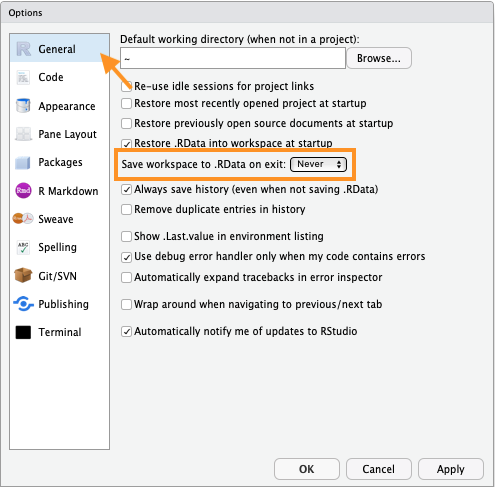
\includegraphics{images/rstudio-on-exit}
  \caption{Réglage de RStudio pour ne pas sauvegarder l'espace
    de travail de R au moment de quitter l'application}
  \label{fig:rstudio:rstudio-on-exit}
\end{figure}

\begin{figure}
  \centering
  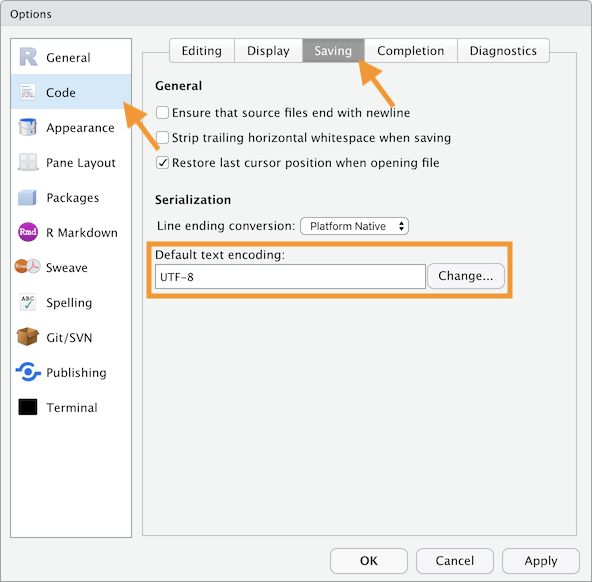
\includegraphics{images/rstudio-utf-8}
  \caption{Réglage de RStudio pour enregistrer les fichiers dans
    l'encodage UTF-8}
  \label{fig:rstudio:rstudio-utf-8}
\end{figure}


\section{Aide et documentation}
\label{sec:rstudio:aide}

La documentation de RStudio se trouve entièrement en ligne. On y
accède par le menu \code{Help}. L'onglet \code{Help} du navigateur de
fichiers (sous-fenêtre en bas à droite) offre également une interface
unifiée pour accéder à l'aide de R et à celle de RStudio.

\index{RStudio|)}

%%% Local Variables:
%%% mode: latex
%%% TeX-engine: xetex
%%% TeX-master: "programmer-avec-r"
%%% coding: utf-8
%%% End:
